\documentclass[12pt,a4paper]{article}
\usepackage[utf8]{inputenc}
\usepackage[spanish,es-tabla]{babel}
\usepackage{geometry}
\usepackage{graphicx}
\usepackage{multirow}
\usepackage{tabularx}
\usepackage{mathptmx}
\usepackage{fancyhdr}
\usepackage{array}
\usepackage[table]{xcolor}
\usepackage{titlesec}
\usepackage{setspace}
\usepackage{microtype}
\usepackage{lastpage}
\usepackage{booktabs}
\usepackage{enumitem}
\usepackage{amsmath}
\usepackage{amsfonts}
\usepackage{amssymb}

\graphicspath{{images/}{../images/}{./}}

\geometry{
    top=4.7cm,
    bottom=2.5cm,
    left=2.5cm,
    right=2.5cm,
    headheight=3.9cm,
    headsep=0.4cm
}

\setstretch{1.15}
\setlength{\parindent}{0pt}
\setlength{\parskip}{0.45em}
\setlength{\tabcolsep}{4pt}

\titleformat{\section}
  {\normalfont\fontsize{12}{14.5}\bfseries}{\thesection.}{0.6em}{\uppercase}
\titlespacing*{\section}
  {0pt}{1.8ex plus 0.4ex minus 0.2ex}{0.6ex plus 0.2ex}

\titleformat{\subsection}
  {\normalfont\fontsize{11.5}{13.5}\bfseries}{\thesubsection.}{0.5em}{}
\titlespacing*{\subsection}
  {0pt}{1.4ex plus 0.3ex minus 0.1ex}{0.4ex plus 0.1ex}

\titleformat{\subsubsection}
  {\normalfont\fontsize{10.5}{12.5}\bfseries\itshape}{\thesubsubsection.}{0.4em}{}
\titlespacing*{\subsubsection}
  {0pt}{1.1ex plus 0.2ex minus 0.1ex}{0.3ex plus 0.1ex}

\newcolumntype{Y}{>{\centering\arraybackslash}X}
\newcolumntype{L}{>{\raggedright\arraybackslash}X}
\newcolumntype{C}{>{\centering\arraybackslash}X}

\definecolor{headerred}{RGB}{180, 0, 0}
\definecolor{darkred}{RGB}{140, 0, 0}
\definecolor{lightgraybg}{RGB}{248, 248, 248}
\definecolor{tableheader}{RGB}{232, 238, 246}

\newcommand{\docCodigo}{TI-SIGE-ENT-S2-003}
\newcommand{\docVersion}{1.0}
\newcommand{\docProceso}{DISEÑO DE SOFTWARE / MODELADO DINÁMICO Y ESTRUCTURAL}
\newcommand{\docElaboracion}{01/09/2026}
\newcommand{\docRevision}{PENDIENTE DE REVISIÓN}
\newcommand{\docTitulo}{DIAGRAMAS UML DE SECUENCIA, ACTIVIDADES Y CLASES DEL DOMINIO}
\newcommand{\docOrganizacion}{FACULTAD DE INGENIERÍA EN SISTEMAS, ELECTRÓNICA E INDUSTRIAL}
\newcommand{\docSubOrganizacion}{CARRERA DE INGENIERÍA DE SOFTWARE}

\newcommand{\encabezadofrecuente}{%
    \renewcommand{\arraystretch}{1.15}%
    \noindent\makebox[\textwidth][c]{%
    \begin{tabularx}{\textwidth}{|>{\centering\arraybackslash}m{2.8cm}|Y|>{\centering\arraybackslash}m{4.8cm}|}
        \hline
        \multirow{4}{2.8cm}{\centering\raisebox{-1.15cm}{
\includegraphics[width=2.5cm,height=2.0cm,keepaspectratio]{images/logo.png}}}
        & \textbf{\fontsize{9}{11}\selectfont \docOrganizacion} 
        & \textbf{\fontsize{8}{10}\selectfont CÓDIGO:} \fontsize{8}{10}\selectfont \docCodigo \\
        \cline{3-3}
        & \textbf{\fontsize{8.5}{10.5}\selectfont \docSubOrganizacion} 
        & \textbf{\fontsize{8}{10}\selectfont VERSIÓN:} \fontsize{8}{10}\selectfont \docVersion \\
        \cline{2-3}
        & \textbf{\fontsize{8}{10}\selectfont PROCESO:} \fontsize{8}{10}\selectfont \docProceso 
        & \textbf{\fontsize{8}{10}\selectfont ELABORACIÓN:} \fontsize{8}{10}\selectfont \docElaboracion \\
        \cline{2-3}
        & \textbf{\fontsize{8.5}{10.5}\selectfont \docTitulo} 
        & \textbf{\fontsize{8}{10}\selectfont ÚLTIMA REVISIÓN:} \fontsize{8}{10}\selectfont \textbf{\textcolor{darkred}{\docRevision}} \\
        \hline
    \end{tabularx}%
    }%
}

\pagestyle{fancy}
\fancyhf{}
\fancyhead[C]{\encabezadofrecuente}
\fancyfoot[C]{\fontsize{10}{12}\selectfont Página \thepage\ de \pageref{LastPage}}
\renewcommand{\headrulewidth}{0pt}

\begin{document}

\section{Título}
\textbf{Denominación del Entregable:} Modelado Dinámico y Estructural del Dominio en UML 2.5: Cascada de Firmas con FirmaEC, Ciclo de Vida Documental y Clases de Dominio.

\vspace{0.15cm}
\noindent
\textbf{Ficha Técnica de Identificación:}
\begin{itemize}[leftmargin=1.5em, itemsep=1.5pt, topsep=1.5pt]
    \item \textbf{Código Documental:} \docCodigo \quad | \quad \textbf{Versión:} \docVersion
    \item \textbf{Institución:} Universidad Técnica de Ambato (UTA) -- FISEI
    \item \textbf{Carrera:} Ingeniería de Software (Séptimo Semestre "A")
    \item \textbf{Módulo Académico:} Gestión de Proyectos de Software
    \item \textbf{Docente Tutor:} Ing. Paulo Torres
    \item \textbf{Fecha de Elaboración:} \docElaboracion \quad | \quad \textbf{Estado:} \textbf{\textcolor{darkred}{En Elaboración / Pendiente de Revisión}}
    \item \textbf{Período de Ejecución:} Semana 2 (27/08/2026 al 02/09/2026 -- EDT 2.3: 5 días hábiles, 40h)
\end{itemize}

\section{Introducción}
El modelado dinámico y estructural formaliza la interacción temporal de objetos, el flujo de mensajes y la jerarquía de clases que sustentan la lógica del sistema \textbf{SIGE}. Este documento detalla los diagramas UML de **Secuencia** (destacando el subsistema criptográfico de firmas electrónicas multinivel con FirmaEC), **Actividades** (ciclo de vida del plan e informe SGC con habilitaciones extemporáneas) y **Clases del Dominio** (entidades, agregados y value objects).

\section{Objetivo}

\subsection{Objetivo General}
Representar formalmente el flujo dinámico de mensajes, el circuito jerárquico de firmas electrónicas en cascada y la estructura estática del dominio de SIGE mediante el estándar UML 2.5.

\subsection{Objetivos Específicos}
\begin{itemize}[leftmargin=1.5em, itemsep=1.5pt, topsep=1.5pt]
    \item Modelar el Diagrama de Secuencia de la Cascada de 3 Firmas Oficiales de la FISEI (Docente $\rightarrow$ Coord. Área $\rightarrow$ Coord. Carrera) integrando el aplicativo estatal FirmaEC y certificados X.509 (.p12).
    \item Formalizar el flujo de validación determinista de matrices, habilitación extemporánea por el Administrador y solicitudes de modificación.
    \item Estructurar el Diagrama de Actividades para la ejecución continua y carga inmediata de evidencias a MinIO.
    \item Detallar el Diagrama de Clases del Dominio con operaciones, tipos e invariantes de negocio.
\end{itemize}

\section{Alcance}

\subsection{Límites del Modelado}
Modela las interacciones entre los actores del SGC (Docente Responsable, Coordinador de Área, Coordinador de Carrera, Administrador), el cliente frontend, la WebAPI en .NET 9, el validador determinista, el almacenamiento de objetos MinIO S3 y el motor criptográfico FirmaEC.

\subsection{Exclusiones}
No modela la comunicación interna de bajo nivel de los drivers criptográficos de tokens físicos ni pasarelas financieras ajenas a la UTA.

\section{Definiciones}
\begin{itemize}[leftmargin=1.5em, itemsep=2pt, topsep=2pt]
    \item \textbf{FirmaEC:} Aplicativo oficial del MINTEL para estampado y verificación de firmas electrónicas X.509.
    \item \textbf{Cascada de Firmas:} Secuencia jerárquica estricta donde cada escalón valida criptográficamente la conformidad del escalón precedente.
    \item \textbf{Validation Gate:} Compuerta lógica determinista en backend que bloquea transiciones de estado si los requisitos no se cumplen al 100\%.
\end{itemize}

\section{Responsabilidades}
\begin{itemize}[leftmargin=1.5em, itemsep=2pt, topsep=2pt]
    \item \textbf{Steeven Toala (Líder / Arquitecto):} Modelado de diagramas de secuencia, protocolo de firmas y arquitectura limpia.
    \item \textbf{Heidy Villavicencio (Analista / UI-UX):} Diagrama de actividades, reglas del formato SGC y verificación de usabilidad.
    \item \textbf{Ing. Paulo Torres (Docente Tutor):} Supervisión y validación técnica del apego a la normativa institucional.
\end{itemize}

\section{Normativa Legal y Técnica}
\begin{itemize}[leftmargin=1.5em, itemsep=2pt, topsep=2pt]
    \item \textbf{Ley de Comercio Electrónico, Firmas Electrónicas y Mensajes de Datos (Ecuador):} Validez probatoria de firmas digitales.
    \item \textbf{OMG UML Specification v2.5.1:} Estándar internacional de modelado de software.
\end{itemize}

\section{Método, Políticas y Contenidos}

\subsection{Diagrama de Secuencia 1: Cascada de Firmas al Inicio (Aprobación de Planificación)}
Modela el flujo oficial en cascada para la legalización del Plan de Trabajo (\texttt{UTA-SGC-A-2-1-P7-T1}). Ningún documento transiciona al estado \texttt{EN\_EJECUCION} sin haber completado los 3 escalones:

\begin{figure}[htbp]
    \centering
    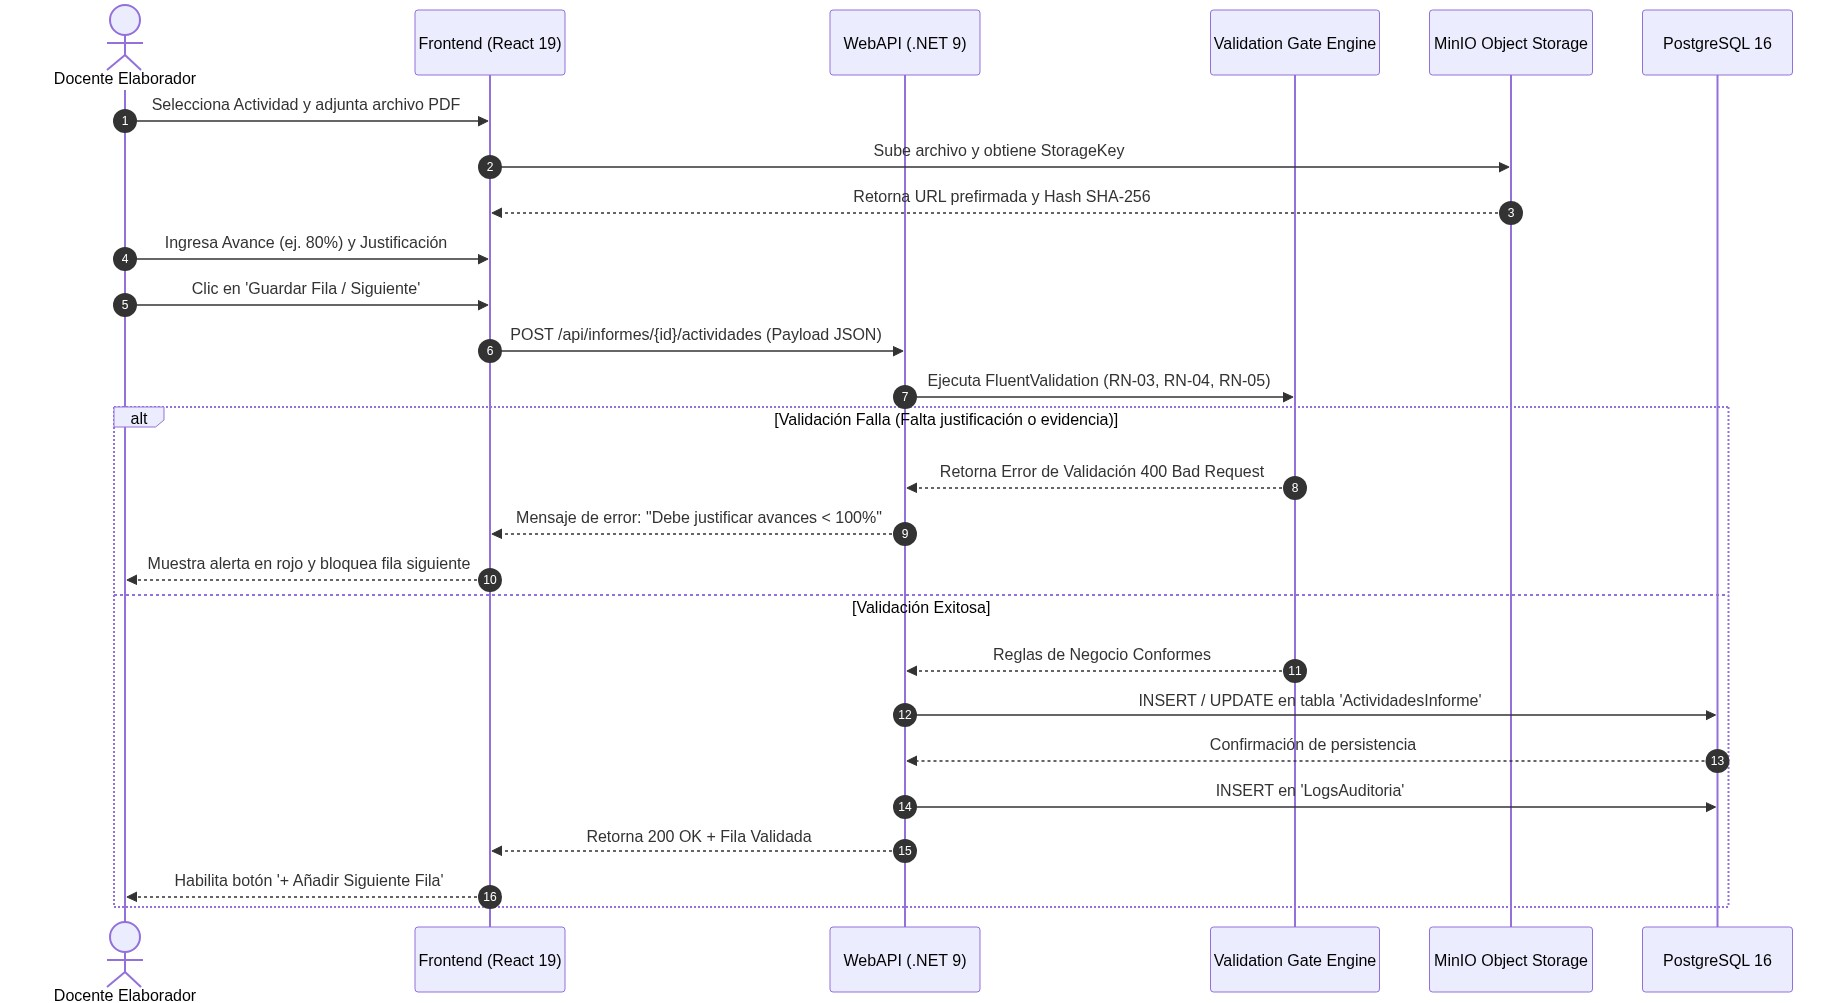
\includegraphics[width=0.92\textwidth,keepaspectratio]{images/s2_03_secuencia_validation.png}
    \caption{Diagrama de Secuencia UML: Cascada de Firmas con FirmaEC y Validación Determinista.}
    \label{fig:s2_03_seq}
\end{figure}

\subsubsection{Detalle del Protocolo Criptográfico con FirmaEC}
\begin{enumerate}[leftmargin=1.5em, itemsep=1.5pt]
    \item \textbf{Escalón 1 -- Elaborado por (Docente Responsable):}
    El docente completa la matriz con el 100.00\% de ponderaciones. Al solicitar firma (\texttt{POST /api/planes/\{id\}/firmas/docente}), la WebAPI calcula el hash SHA-256 del expediente. El docente firma mediante el componente FirmaEC con su certificado \texttt{.p12}. Se almacena el sello digital Base64 en la tabla \texttt{FIRMAS\_LEGALIZACION} (Orden 1), se promueve el documento a \texttt{PLAN\_PENDIENTE\_FIRMA\_COORD\_AREA} y se bloquea la edición al docente.
    
    \item \textbf{Escalón 2 -- Revisado por (Coordinador de Área de Conocimiento):}
    El Coordinador de Área inspecciona la articulación académica. Si detecta inconsistencias, rechaza registrando observaciones, lo que rompe la cascada y retorna el documento a \texttt{PLAN\_OBSERVADO\_DEVUELTO}. Si aprueba, invoca \texttt{POST /api/planes/\{id\}/firmas/coordinador-area}. La WebAPI verifica como precondición estricta que la Firma 1 esté en estado \texttt{FIRMADO}. Se estampa la segunda firma electrónica y avanza a \texttt{PLAN\_PENDIENTE\_FIRMA\_COORD\_CARRERA}.
    
    \item \textbf{Escalón 3 -- Aprobado por (Coordinador de Carrera):}
    El Coordinador de Carrera verifica la pertinencia curricular. Al aprobar (\texttt{POST /api/planes/\{id\}/firmas/coordinador-carrera}), la API valida la existencia y validez de la Firma 1 y Firma 2. Se estampa la 3ra firma legalizando el expediente en \texttt{PLAN\_APROBADO\_Y\_LEGALIZADO}, transicionando automáticamente a \texttt{EN\_EJECUCION}.
\end{enumerate}

\subsection{Diagrama de Actividades: Ciclo de Vida Documental Integral SGC}
El diagrama formaliza el flujo de extremo a extremo, incluyendo la habilitación extemporánea otorgada por el Administrador con plazo de gracia, el trámite de solicitudes de modificación de matriz durante el semestre y la carga oportuna de evidencias digitales en MinIO S3 inmediatamente al culminar cada actividad.

\begin{figure}[htbp]
    \centering
    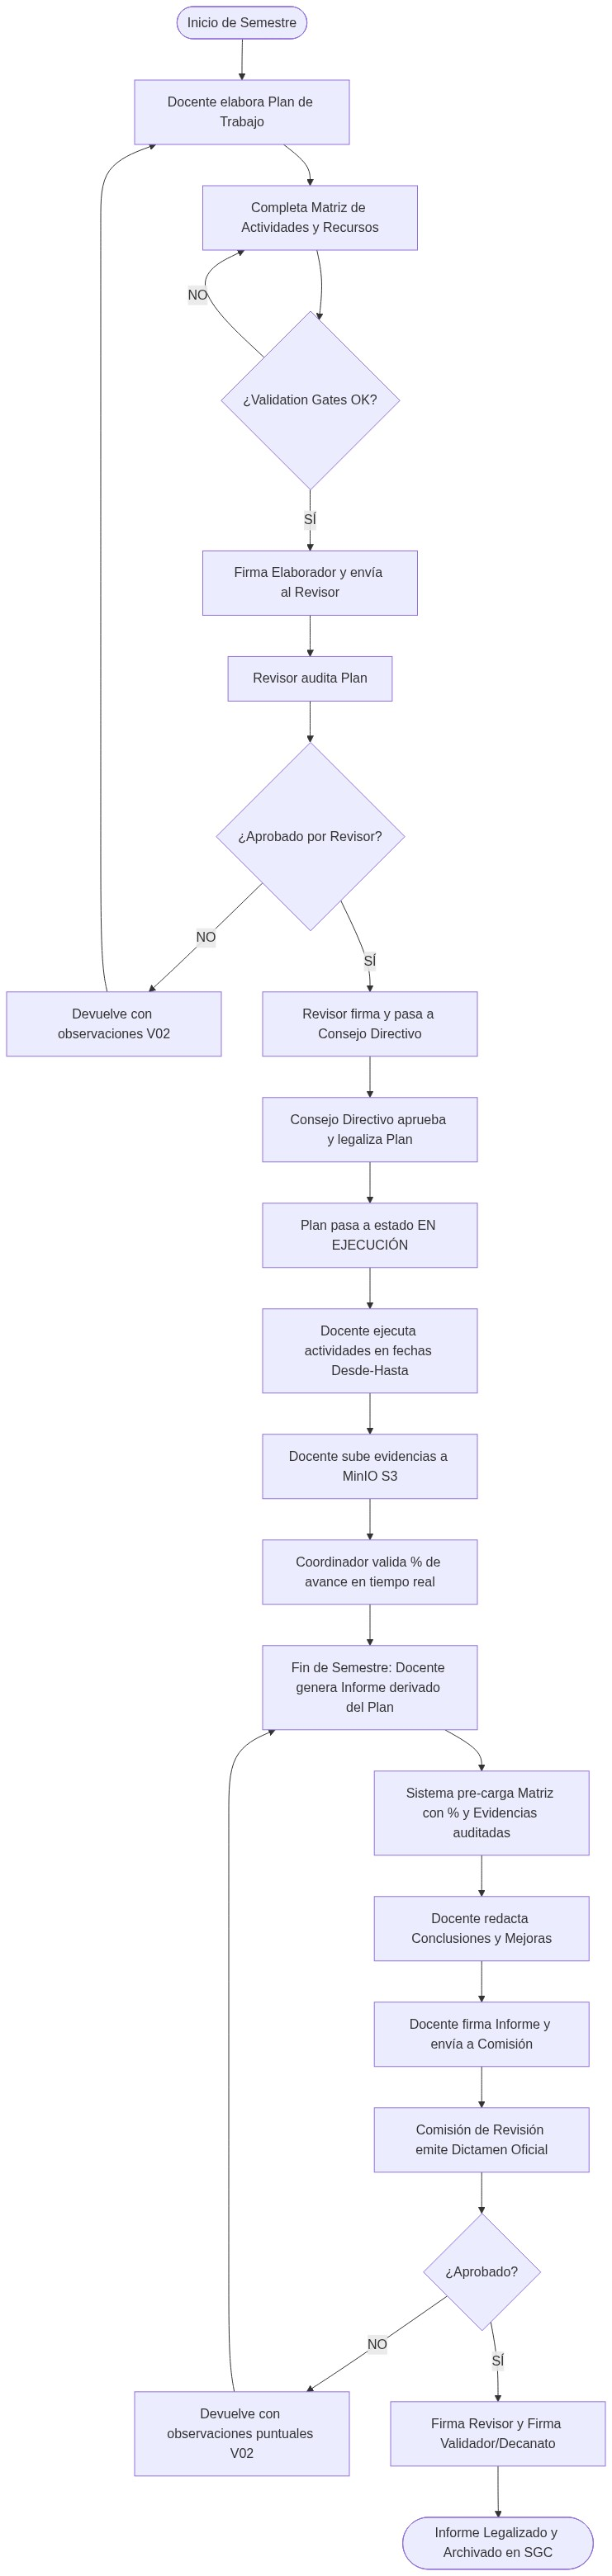
\includegraphics[width=0.75\textwidth,keepaspectratio]{images/s2_03_actividades_ciclo.png}
    \caption{Diagrama de Actividades UML: Ciclo Completo del Plan e Informe SGC en SIGE.}
    \label{fig:s2_03_act}
\end{figure}

\section{Descripción de actividades y Modelado Estático}

\subsection{Diagrama de Clases del Núcleo de Dominio}
Representa las entidades centrales del dominio, tipos fuertemente tipados e invariantes de negocio:

\begin{figure}[htbp]
    \centering
    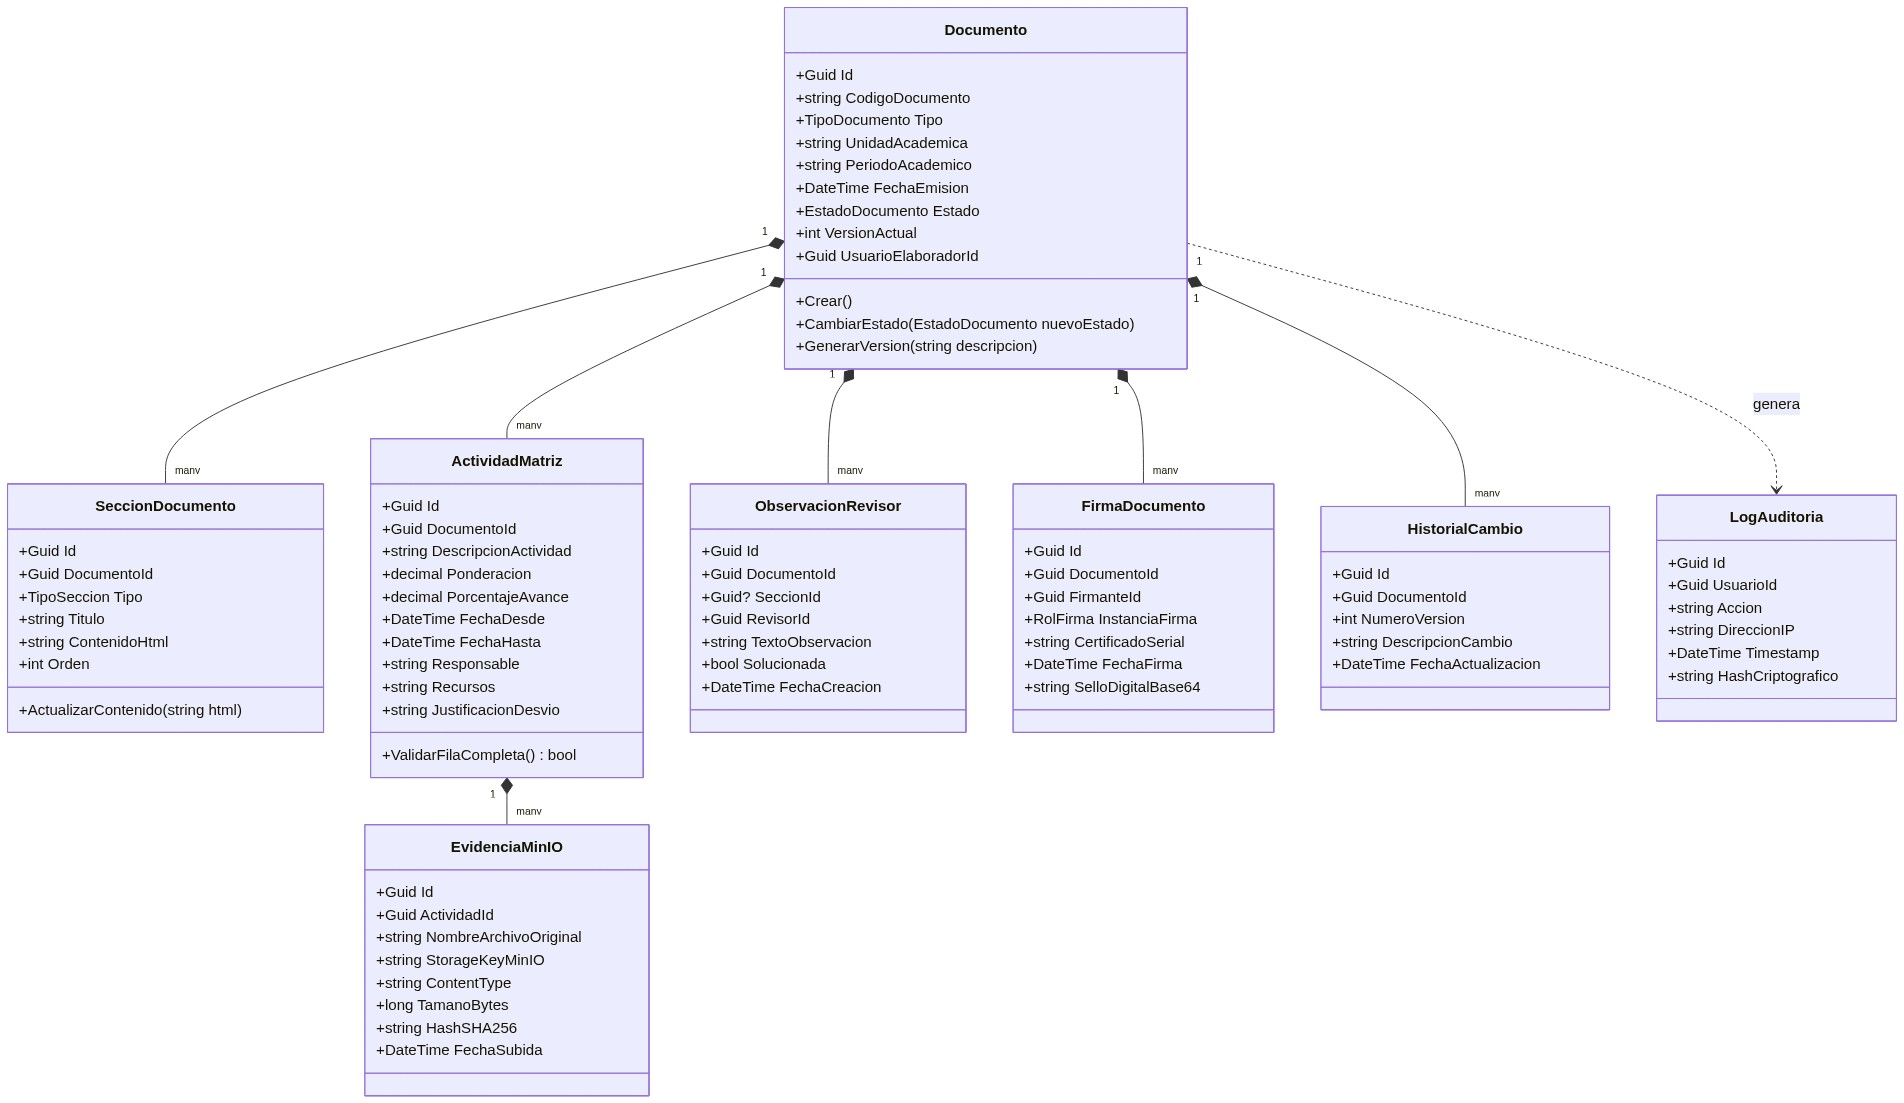
\includegraphics[width=0.92\textwidth,keepaspectratio]{images/s2_03_clases_uml.png}
    \caption{Diagrama de Clases UML del Dominio SIGE.}
    \label{fig:s2_03_clases}
\end{figure}

\subsubsection{Responsabilidades de las Clases del Dominio}
\begin{itemize}[leftmargin=1.5em, itemsep=2pt]
    \item \textbf{Documento:} Agregado raíz que encapsula la máquina de estados, el versionamiento y la foliación oficial.
    \item \textbf{ItemActividadMatriz:} Representa cada fila de la matriz oficial SGC (ponderación, porcentaje de ejecución, fechas desde/hasta, recursos y medios de verificación).
    \item \textbf{FirmaCascada:} Entidad inmutable que registra el escalón jerárquico (1, 2, 3), el sello Base64, el serial del certificado y valida la precedencia estricta.
    \item \textbf{EvidenciaMinIO:} Representa los medios probatorios almacenados de forma segura con hash SHA-256 inmutable.
\end{itemize}

\section{Conclusiones}
\begin{itemize}[leftmargin=1.5em, itemsep=2pt]
    \item El modelado dinámico formaliza con rigor matemático el flujo de validación y la cascada inmutable de firmas con FirmaEC, impidiendo firmas desordenadas o adulteraciones.
    \item La estructura de clases y actividades garantiza la total fidelidad con los formatos oficiales \texttt{UTA-SGC-A-2-1-P7-T1} y \texttt{UTA-SGC-A-2-1-P7-T2}.
\end{itemize}

\section{Recomendaciones}
\begin{itemize}[leftmargin=1.5em, itemsep=2pt]
    \item Implementar las precondiciones de cascada mediante validadores FluentValidation y constraints a nivel de base de datos relacional.
\end{itemize}

\section{Referencias Bibliográficas}
\begin{itemize}[leftmargin=1.5em, itemsep=2pt]
    \item Booch, G., Rumbaugh, J., \& Jacobson, I. (2005). \textit{The Unified Modeling Language User Guide}. Addison-Wesley.
    \item MINTEL. (2025). \textit{Manual Técnico de Integración FirmaEC}. Quito, Ecuador.
\end{itemize}

% =============================================================
% FIRMAS DE RESPONSABILIDAD
% =============================================================
\section{Firmas de Responsabilidad}

\noindent
\renewcommand{\arraystretch}{1.2}
\begin{tabularx}{\textwidth}{|>{\raggedright\arraybackslash}m{2.9cm}|>{\raggedright\arraybackslash}X|>{\centering\arraybackslash}m{4.6cm}|>{\centering\arraybackslash}m{2.3cm}|}
    \hline
    \rowcolor{headerred}
    \textcolor{white}{\textbf{ACCIÓN}} & \textcolor{white}{\textbf{NOMBRE Y CARGO}} & \textcolor{white}{\textbf{FIRMA}} & \textcolor{white}{\textbf{FECHA}} \\
    \hline
    \textbf{Elaborado por:} & Steeven Toala\newline \textit{Líder de Proyecto / Arquitecto Software} & \parbox[c]{4.4cm}{\centering\vspace{4pt}
\includegraphics[height=1.5cm,width=4.0cm,keepaspectratio]{images/firma_steveen.png}\vspace{4pt}} & 01/09/2026 \\
    \hline
    \textbf{Revisado por:} & Heidy Villavicencio\newline \textit{Analista de Requerimientos / UI-UX} & \parbox[c]{4.4cm}{\centering\vspace{4pt}
\includegraphics[height=1.5cm,width=4.0cm,keepaspectratio]{images/firma_heidi.png}\vspace{4pt}} & 01/09/2026 \\
    \hline
    \textbf{Aprobado por:} & Ing. Paulo Torres\newline \textit{Docente Tutor - Gestión Proyectos Software} & \parbox[c]{4.4cm}{\centering\vspace{10pt}\textbf{\textcolor{gray!80}{\scriptsize [ PENDIENTE DE APROBACIÓN ]}}\vspace{10pt}} & \textbf{\textcolor{gray!90}{Pendiente}} \\
    \hline
\end{tabularx}

\vspace{0.4cm}

% =============================================================
% CONTROL DE CAMBIOS
% =============================================================
\section{Control de Cambios}

\noindent
\renewcommand{\arraystretch}{1.2}
\begin{tabularx}{\textwidth}{|>{\hsize=0.45\hsize\centering\arraybackslash}X|>{\hsize=1.55\hsize\raggedright\arraybackslash}X|>{\hsize=1.2\hsize\raggedright\arraybackslash}X|>{\hsize=0.8\hsize\centering\arraybackslash}X|}
    \hline
    \rowcolor{gray!20}
    \textbf{Versión} & \textbf{Descripción del cambio} & \textbf{Responsable del cambio} & \textbf{Fecha de aprobación} \\
    \hline
    1.0 & Modelado completo de secuencia con FirmaEC, actividades y clases de dominio para Séptimo Semestre "A" & Steeven Toala & 01/09/2026 \\
    \hline
\end{tabularx}

\end{document}


